\chapter{Cloud Deployment Procedure}
\label{chap:deployment}

\section{Step-by-Step Deployment Pipeline}
The deployment process follows a systematic multi-phase sequence:

\subsection{Phase 1: VPC and Relational Database Provisioning}
\begin{enumerate}
    \item Provision Amazon VPC with CIDR \texttt{10.0.0.0/16}, creating 2 Public Subnets and 2 Private Subnets across \texttt{us-east-1a} and \texttt{us-east-1b}.
    \item Create DB Subnet Group associating private subnets.
    \item Launch Amazon RDS for PostgreSQL instance (\texttt{cloudcampus-db}) on PostgreSQL 15.3 using \texttt{db.t4g.micro} class.
    \item Configure Security Group \texttt{sg-cloudcampus-db} allowing TCP 5432 ingress only from Lambda security group.
\end{enumerate}

\subsection{Phase 2: Database Schema Migration and Seeding}
\begin{enumerate}
    \item Execute Prisma Client generation: \texttt{npx prisma generate}.
    \item Push database schema definitions: \texttt{npx prisma db push}.
    \item Execute seed script: \texttt{npx ts-node prisma/seed.ts} to populate baseline departments, faculty, students, and course catalogs.
\end{enumerate}

\subsection{Phase 3: AWS Lambda Backend Packaging and Deployment}
\begin{enumerate}
    \item Compile TypeScript backend source code to JavaScript: \texttt{npm run build}.
    \item Package distribution directory \texttt{dist/} and production dependencies into a deployment zip archive.
    \item Deploy code to AWS Lambda function \texttt{cloudcampus-backend-api} via AWS CLI:
    \begin{verbatim}
    aws lambda update-function-code \
      --function-name cloudcampus-backend-api \
      --zip-file fileb://backend-dist.zip
    \end{verbatim}
    \item Configure environment variables (\texttt{DATABASE\_URL}, \texttt{JWT\_SECRET}, \texttt{UPLOAD\_DIR}).
\end{enumerate}

\subsection{Phase 4: API Gateway Integration}
\begin{enumerate}
    \item Create REST API in API Gateway named \texttt{CloudCampus-REST-API}.
    \item Configure \texttt{/api/\{proxy+\}} route with HTTP proxy integration invoking Lambda backend.
    \item Enable CORS pre-flight headers and deploy stage to \texttt{production}.
\end{enumerate}

\subsection{Phase 5: S3 Static Frontend Deployment}
\begin{enumerate}
    \item Build production React SPA bundle: \texttt{npm run build} in \texttt{frontend/}.
    \item Sync compiled assets in \texttt{frontend/dist} to S3 bucket:
    \begin{verbatim}
    aws s3 sync frontend/dist/ s3://cloudcampus-frontend-static --delete
    \end{verbatim}
    \item Enable Static Website Hosting with index document \texttt{index.html}.
\end{enumerate}

Figure~\ref{fig:deploy_console} illustrates the AWS Management Console deployment status.

\begin{figure}[htbp]
\centering
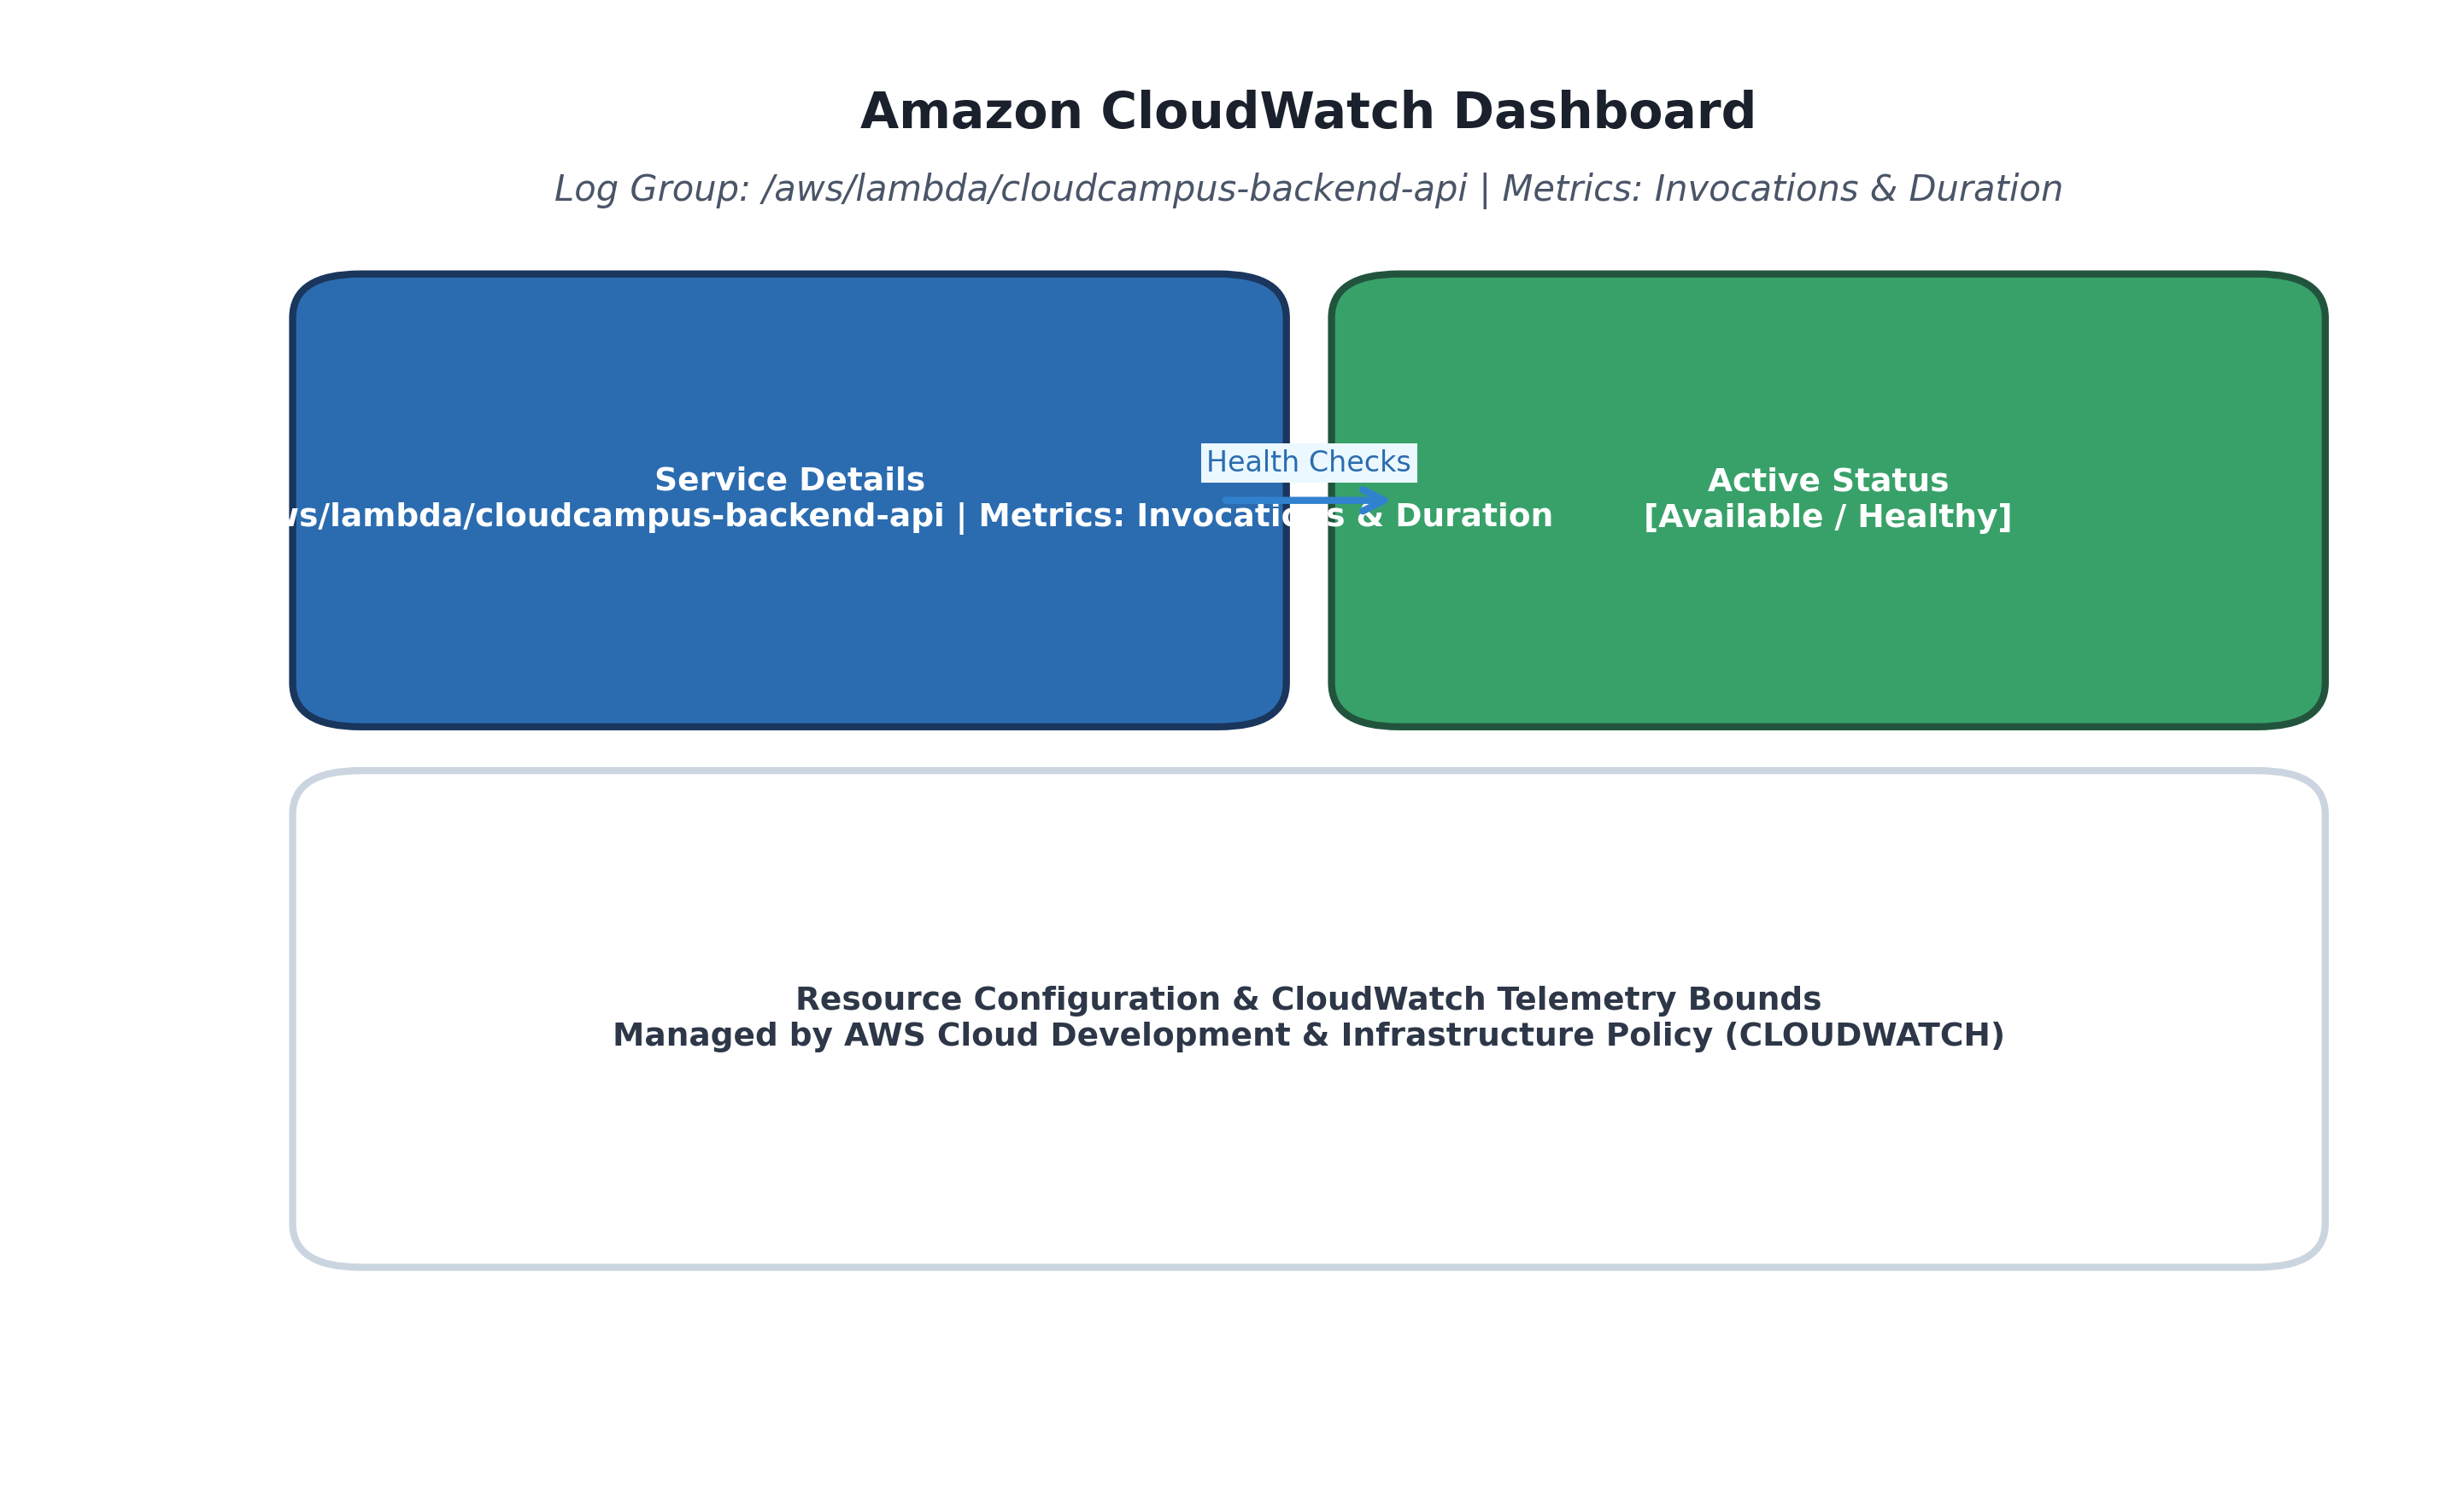
\includegraphics[width=0.88\textwidth]{figures/dashboard.png}
\caption{CloudWatch Monitoring Dashboard for AWS Lambda and RDS Services Console View}
\label{fig:deploy_console}
\end{figure}
